\section{Experiments}

\subsection{Benchmarks}

\subsubsection{Sokoban}

Sokoban is a classic planning problem. It is a challenging one-player puzzle game in which the goal is to navigate a gridworld maze and push boxes onto target tiles. A Sokoban puzzle is considered solved when all boxes are positioned on top of target locations. The player can move in all 4 cardinal directions and only push boxes into an empty space (as opposed to pulling). For this reason many moves are irreversible and mistakes can render the puzzle unsolvable. A human player is thus forced to plan moves ahead of time. Artificial agents should similarly benefit from a learned model and simulation.

Despite its simple ruleset, Sokoban is an incredibly complex game for which no general solver exists. It can be shown that Sokoban is NP-Hard and PSPACE-complete\cite{Theory.Sokoban} \editnote{Revise what does it mean NP-Hard and PSPACE-complete, hehe}. Sokoban has an enormous state space that makes it inassailable to exhaustive search methods. An efficient automated solver for Sokoban must have strong heuristics, just as humans utilize their strong intuition, so that it is not overwhelmed by the number of possible game states.

The implementation of Sokoban\cite{Code.Sokoban} used for those experiments procedurally generates a new level each episode. This means an agent cannot memorize specific puzzles. Together with the planning aspect, this makes for a very challenging environment. While the underlying game logic operates in a 10 × 10 grid world, agents were trained directly on RGB sprite graphics. Fig.~\ref{Fig.Sokoban} shows an example of Sokoban level with 4 boxes and fig.~\ref{Fig.Sokoban_elements} explains the meaning of the visual icons.

\begin{figure}[H]
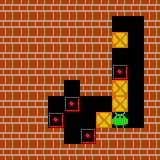
\includegraphics[]{figures/Sokoban.png}
\caption[Sokoban]{Example of Sokoban level (image size 160 × 160 pixels)}
\label{Fig.Sokoban}
\end{figure}

\begin{figure}[H]
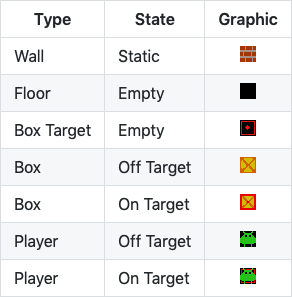
\includegraphics[width=0.5\textwidth,keepaspectratio]{figures/Sokoban_elements.png}
\caption[]{Sokoban level elements}
\label{Fig.Sokoban_elements}
\end{figure}
